\documentclass[a4paper]{article}

\usepackage[english]{babel}
\usepackage[utf8]{inputenc}
\usepackage{amsmath}
\usepackage{graphicx}
\usepackage{hyperref}
\usepackage[colorinlistoftodos]{todonotes}

\title{Machine Learning Nanodegree  \linebreak Capstone Proposal}

\author{Marcelo Roger García Escalante}

\date{\today}

\begin{document}
\maketitle

\section{Domain Background}
Machine learning, in layman terms, consists of programming the computer to learn from previous data. A more detail description could be given as stated in \cite{MLState}: "Machine learning is the process (algorithm) of estimating a model that’s true to the real-world problem with a certain probability
from a dataset (or sample) generated by finite observations in a noisy environment."

Today Machine Learning's method Deep Reinforcement Learning is gaining popularity since lots of applications has been given to it, such as Video Games, unmanned vehicles, and control systems. The latter is a well-known field where the goal is to make dynamical systems behave in a desired manner, to achieve this it is required to obtain the mathematical model of the system as explained in \cite{Control}

Since control systems are dynamic, all its environments are modeled as a continuous state space and most of the times as a continuous action space as well. Therefore, it signifies a challenging task to solve by machine learning, some of the algorithms able to tackle these problems are deep Q learning (for infinite state spaces and discrete action spaces), and actor-critic methods (for infinite state and action spaces). 

Most of the times it is not possible to know all the system features thus it is not possible to get the mathematical model of the system, that is the main reason why a Reinforcement Learning approach could be useful to solve the problem. One approach of Reinforcement Learning applied to Control systems is presented in "A heuristic approach to reinforcement learning control systems" \cite{1098193}

\subsection{Motivation}
The motivation behind this project is because control is one of the required fields for robotics, in more specific for self-driving cars, where I would love to be involved in. Finally, I am convinced that my previous knowledge of control theory will be enhanced by relating Machine Learning with Control Systems, where there is a lot of room to work in. Therefore my main goal is to enlarge my experience in the combination of Deep Reinforcement Learning with Control Systems.

% Student briefly details background information of the domain from which the project is proposed. Historical information relevant to the project should be included. It should be clear how or why a problem in the domain can or should be solved. Related academic research should be appropriately cited. A discussion of the student's personal motivation for investigating a particular problem in the domain is encouraged but not required.

\section{Problem Statement}
\label{sec:problem-statement}
The project aims to solve an OpenAI gym environment from the control section that can be seen here \href{https://gym.openai.com/envs/#classic_control}{Control Environments}. The environment selected is the MountainCar-v0 because it has a continuous state space with a deterministic action space being a good candidate for applying deep q learning. The details of the problem are as follows:
\begin{itemize}
\item \textbf{Task:} MountainCar-v0
\item \textbf{Category:} Classic Control
\item \textbf{Goal:} Get an under powered car to the top of a hill (top = 0.5 position) by creating momentum as shown in Fig.\ref{fig:car}
\begin{figure}[h]
\centering
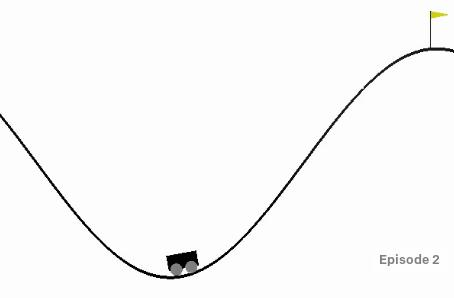
\includegraphics[width=0.8\textwidth]{environment.jpg}
\caption{\label{fig:car} Mountain Car environment}
\end{figure}
\item \textbf{State Space:}
      \begin{table}[h]
      \centering
      \begin{tabular}{|c|c|c|c|}
      \hline
      \textbf{Num} & \textbf{Observation} & \textbf{Min} & \textbf{Max} \\ \hline
      0            & position             & -1.2         & 0.6          \\ \hline
      1            & velocity             & -0.07        & 0.07         \\ \hline
      \end{tabular}
      \caption{State Space}
      \label{tab:1}
      \end{table}
\item \textbf{Action Space:}
		\begin{table}[h]
        \centering
        \begin{tabular}{|c|c|}
        \hline
        \textbf{Num} & \textbf{Observation} \\ \hline
        0            & push left            \\ \hline
        1            & no push              \\ \hline
        2            & push right           \\ \hline
        \end{tabular}
        \caption{Action Space}
        \label{my-label}
        \end{table}
\item \textbf{Termination Criteria:} The episode ends when either the goal is reached or 200 actions are made.
\item \textbf{Rewards:} -1 penalty for each environment step until termination criteria is met.
\item \textbf{Potential Solution:} Since the environment has continuous state space and discrete action space a good candidate would be a \textbf{Deep Q Network}
\end{itemize}
% Student clearly describes the problem that is to be solved. The problem is well defined and has at least one relevant potential solution. Additionally, the problem is quantifiable, measurable, and replicable. 

\section{Datasets and Inputs}
There is no dataset for this project since it involves a Deep Reinforcement Learning approach. However, the inputs for the model will be the states of the environment which in this case are two continuous measurements: position and velocity of the car as shown in \ref{tab:1}.
% The dataset(s) and/or input(s) to be used in the project are thoroughly described. Information such as how the dataset or input is (was) obtained, and the characteristics of the dataset or input, should be included. It should be clear how the dataset(s) or input(s) will be used in the project and whether their use is appropriate given the context of the problem.

\section{Solution Statement}
As explained in \hyperref[sec:problem-statement]{Section
\ref*{sec:problem-statement}} The problem's best candidate is a Deep Q Network, which will have a Circular Memory (Deque) or a tree Memory(sum-tree) in case a prioritize Memory is required. Since the initial state is different in each iteration it may require a tweak of the state obtained from the environment before processing it to the deep network. 

The deep Q network will be in charge of getting the best function to map the state input to one of the three actions, that is seeking for the optimal policy.
% Student clearly describes a solution to the problem. The solution is applicable to the project domain and appropriate for the dataset(s) or input(s) given. Additionally, the solution is quantifiable, measurable, and replicable.

\section{Benchmark Model}
The project will be compared against three benchmarks:
\begin{itemize}
\item \textbf{Random approach}, to ensure the model is better than the most basic model.
\item \textbf{-110 average rewarding}, as stated in \href{https://github.com/openai/gym/wiki/Leaderboard#mountaincar-v0}{OpenAI's documentation} for the MountainCar-v0 the problem pass criteria is a reward of -110 in 100 consecutive episodes
\item \textbf{Leader board}, as explained in the same \href{https://github.com/openai/gym/wiki/Leaderboard#mountaincar-v0}{documentation} there are two algorithms that met the pass criteria as shown in Table\ref{tab:crit}. 

\begin{table}[h]
\centering
\begin{tabular}{|c|c|}
\hline
\textbf{User}      & \textbf{Episodes before solve} \\ \hline
jing582            & 1119                           \\ \hline
DaveLeongSingapore & 1967                           \\ \hline
\end{tabular}
\caption{Leader board for the MountainCar-V0 problem}
\label{tab:crit}
\end{table}

\end{itemize}
% A benchmark model is provided that relates to the domain, problem statement, and intended solution. Ideally, the student's benchmark model provides context for existing methods or known information in the domain and problem given, which can then be objectively compared to the student's solution. The benchmark model is clearly defined and measurable.

\section{Evaluation Metrics}
\textbf{Average Reward} The main metric for the project will be the average reward in 100 consecutive episodes.
\newline
\textbf{Number of episodes} The secondary metric is the number of episodes in which the problem converges to a solution.
% Student proposes at least one evaluation metric that can be used to quantify the performance of both the benchmark model and the solution model presented. The evaluation metric(s) proposed are appropriate given the context of the data, the problem statement, and the intended solution.

\section{Project Design}
In this section, an explanation of the programming language, libraries and the selected algorithm to tackle the problem is given.
\subsection{Programming Language and Libraries}
    \begin{itemize}
    \item \textbf{Python 3.}
    \item \textbf{Scikit-learn}. Open source machine learning library for Python.
    \item \textbf{Keras.} Open source neural network library written in Python. It is capable of
    running on top of either Tensorflow or Theano.
    \item \textbf{TensorFlow.} Open source software libraries for deep learning.
    \item \textbf{OpenAI gym.} Open source framework for testing reinforcement learning projects
    \end{itemize}
    
\subsection{Deep Q Learning algorithm}
As stated in \href{https://storage.googleapis.com/deepmind-media/dqn/DQNNaturePaper.pdf}{DeepMind's paper} the algorithm for the DQN should have the following structure:
\begin{itemize}
\item Initialize replay Memory with capacity N
\item Initialize Main Q-network weights $W$ with random uniform distribution.
\item Initialize Target Q-network weights with the main Q-network weights. $W^-\leftarrow W$
\item \textbf{For} the episode in maximum number of (Episodes):
\begin{itemize}
\item Reset environment
\item Prepare initial state: $S$
\item \textbf{For} time step t in maximum number of (Steps):
\begin{itemize}
\item[] \underline{\textbf{Observation stage (sample to memory)}}
\item Act in the environment based on state $S$ and get action $A$ using an epsilon-greedy algorithm
\item Take action $A$ and make an environment action-step, get from the output of the environment the new state $S'$ and reward $R$
\item Store the tuple ($S,A,R,S'$) in memory
\item update state. $S \leftarrow S'$
\item[] \underline{\textbf{Learning stage }}\textbf{\dots} 
\item Obtain random mini-batch of tuples from memory. list of ($S,A,R,S'$).
\item Use Target Q-Network to predict the target $Q$ for Main Q-Network for each tuple of the mini-batch. 

$\hat{Q}$=predict($S$)

$\hat{Q}[A]=R+\gamma argMax_a(Q[S',W^-])$
\item Update weights in the Main Q-Network based on the target $\hat{Q}$ as follows: 

$\Delta W=\alpha (Q-\hat{Q}) \nabla_W(\hat{Q})$
\item Update Target Q-network weights with the Main Q-network weights every C steps. $W^-\leftarrow W$
\end{itemize}
\end{itemize}
\end{itemize}
% Student summarizes a theoretical workflow for approaching a solution given the problem. Discussion is made as to what strategies may be employed, what analysis of the data might be required, or which algorithms will be considered. The workflow and discussion provided align with the qualities of the project. Small visualizations, pseudocode, or diagrams are encouraged but not required.
\vspace*{1cm}
\bibliographystyle{plainnat}
\bibliography{bibliography}
\end{document}